% Figure from MATH 556 notes, section 20. Compile with the notes preamble.
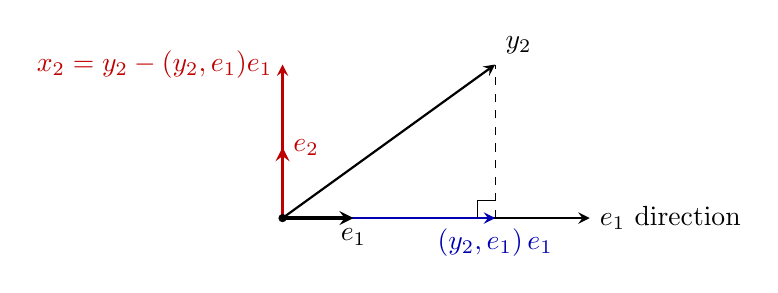
\begin{tikzpicture}[scale=1.5, >=stealth]
    \draw[->, thick] (0,0) -- (2.6,0) node[right] {$e_1$ direction};
    \draw[->, thick] (0,0) -- (1.8,1.3) node[above right] {$y_2$};
    \draw[->, thick, blue!70!black] (0,0) -- (1.8,0) node[below, blue!70!black] {$(y_2, e_1)\, e_1$};
    \draw[dashed] (1.8,0) -- (1.8,1.3);
    \draw (1.65,0) -- (1.65,0.15) -- (1.8,0.15);
    \draw[->, thick, red!75!black] (0,0) -- (0,1.3) node[left, red!75!black] {$x_2 = y_2 - (y_2, e_1) e_1$};
    \draw[->, very thick, red!75!black] (0,0) -- (0,0.6) node[right, red!75!black] {$e_2$};
    \draw[->, very thick] (0,0) -- (0.6,0) node[below] {$e_1$};
    \fill (0,0) circle (1pt);
\end{tikzpicture}
